%% V1.0
%% by Mahmoud Selim, mahmoudahmedselim96@gmail.com

%% Be Udacious!

\documentclass[10pt,journal,compsoc]{IEEEtran}

\usepackage[pdftex]{graphicx}    
\usepackage{cite}
\hyphenation{op-tical net-works semi-conduc-tor}


\begin{document}

\title{Slam In Robotics}

\author{Mahmoud Selim}

\markboth{SLAM project, Robotic Nanodegree, Udacity, RTAB\_Mapping, Robotics}%
{}
\IEEEtitleabstractindextext{%

\begin{abstract}
In Robotics, localization and mapping are the key skills that enable robots to interact with their environment, by being able
to locate itself relative to the map of previously visited locations. Mapping a location (e.g. an apartment room or an outdoor area) from
sensor data while locating oneself in that consistently updating environment is referred to as Simultaneous Localization And Mapping
(SLAM). In this project the SLAM implementation of Real-Time Appearance Based Mapping (RTABMap) is done through the
rtabmap\_ros package and implemented on a teleoperated robot to map 2 simulated worlds made in Gazebo. Both worlds were
successfully mapped, which allows for a first look at some considerations to be made when attempting to map an environment using
robots.
\end{abstract}

% Note that keywords are not normally used for peerreview papers.
\begin{IEEEkeywords}
Robot, IEEEtran, Udacity, deep learning.
\end{IEEEkeywords}}


\maketitle
\IEEEdisplaynontitleabstractindextext
\IEEEpeerreviewmaketitle
\section{Introduction}
\label{sec:introduction}

\IEEEPARstart{T}{he} goal of this project is to perform simultaneos localization and mapping for two environments using the RTABMap algorithm implemented on. SLAM in
robotics enables a robot to map an environment and also to keep track of the position relative to the environment it
is in.
More often than not, the architect blueprint of a building
is inaccurate, and even in the event that it was perfectly
accurate, the addition of furniture would alter the ”map” of
the building by the robot, since if it were to perform a task
within that environment, it would need to know about the
position of this furniture.
This problem is interesting because it implies that every building needs to be mapped if a robot is going to do anything
autonomously within these buildings. This statement can be pushed further to
encompass any kind of environments. However in the ideal situation, the 
robot will adapt it's map when slight changes occurs within it.
Therefore, if one can make a robot able to navigate and
sense it's surroundings, then these environments should be mapped.

Potential applications can go from mapping an office
layout for automated cleaning, mapping a suburb for civil
engineers to design upgrades to a city, to mapping a region
of the moon for installing a base on the moon. The importance of mapping is similar to how important it is for humans
to remember places they’ve been to. Thus, it is a crucial part for any mobile robot to not only be able to map its environment, but also to adjust these maps when changes occurs to them.



\section{BACKGROUND}
\subsection{Mapping in Robotics}
Mapping in Robotics is used to enable the robot to model the environment it is in. Locating the robot with respect
to its environment requires a map of the environment, and
mapping requires the robot’s pose, which is obtained during
the localization. This is a typical scenario for the ”chicken and the egg”
problem, where location requires a map of the environment to be referenced to
and mapping requires the location of the robot.
\subsection{SLAM}
Simultaneous Localization and Mapping (SLAM) solves this
problem by simultaneously and iteratively computing the
map (m) and robot’s pose (x\_t) from sensory and odometric measurements (z\_t), control actions (u\_t), and correspondences (c\_t) between features within the map. There are two
different variants of SLAM:
\begin{itemize}
\item Online SLAM: it solves the SLAM problem by only
looking at the current pose and local correspondences to estimate the robot’s pose and update the
map: P(x\_t, m, c\_t|u\_{1:t}, z\_{1:t}).
\item Full SLAM: Unlike the Online SLAM, Full SLAM,
also referred to Offline SLAM, takes into account all
poses and map correspondences to estimate the pose
and update the map: P(x\_{1:t}, m, c\_{1:t}|u\_{1:t}, z\_{1:t}).
\end {itemize}
There exist different implementations of the SLAM algorithm, examples for these might be FastSLAM, Grid-Based
SLAM, and Graph SLAM.

\paragraph FastSLAM estimates the pose of the robot using particles, like the Monte Carlo Localization algorithm and builds
the map using an EKF to solve the independent features
of the map as local Gaussians. The main disadvantage of
this approach is that it always need to assume that there
are known landmarks within the map, and therefore it is
impossible to model an arbitrary environment.
\paragraph Grid-Based SLAM is a variant of FastSLAM which
updates the map using grids, like the Occupancy Grid Mapping algorithm, in order to fix the previously mentioned
issues with the FastSLAM algorithm. Grid-Based SLAM,
like FastSLAM uses a particle filter to estimates the pose
\paragraph GraphSLAM on the other hand aims create a graph of
robot poses and map features and attempts to minimize the
over error between all motion and measurement constraints.

\subsection{RTABMap}
\subsubsection{General Description}
Real-Time Appearance Based Mapping (RTABMap) or Appearance Based SLAM implements GraphSLAM by collecting data from visual sensors to locate the robot and map the
environment. SLAM with RTABMap can be separated into
two parts: the front-end, which uses sensory and odometric data to create a graph with loop closure constraints; the
second part, the back-end, handles the graph optimization
and the 2D/3D mapping.

\begin{figure}[thpb]
      \centering
      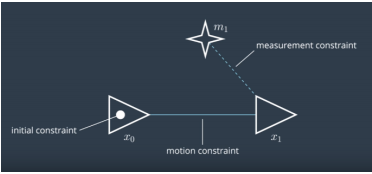
\includegraphics[width=\linewidth]{graph_slam}
      \caption{Graph SLAM Nodes.}
      \label{fig: Graph SLAM}
\end{figure}


\subsubsection{Loop closure and bag-of-words}
RTABMap uses loop closure to determine whether a robot
has seen a location before. RTABMap uses Speeded Up
Robust Features (SURF) to extract features and describe
them with a unique representations then it clusters similar
or synonym features together and name them to create
vocabulary. One of the feature description is then mapped
to one the vocabulary, it is called quantization. Features are
now linked to a word and can be referred to as a visual
word. When all features in an image are quantized, the
image is now a bag-of-words. To compare an image with
previously seen images, a matching score is given to all
images containing the same words using a bayesian filter,
and similar images can be found, this is called an inverted
index. Finally if the current image contains similar words to
that of a previously seen image (bag-of-words) it will have
a higher score, and if the score reaches a threshold H, a loop
closure is detected
\begin{figure}[thpb]
      \centering
      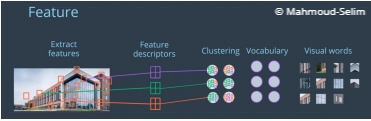
\includegraphics[width=\linewidth]{bag_of_words}
      \caption{ Features are extracted and a bag-of-words is created from an image}
      \label{fig:bow}
\end{figure}

\subsubsection{Memory management}
RTABMap uses a memory management technique to limit
the number of locations considered as candidates during
loop-closure detection, which allows it to be done in RealTime. The technique can be summarized as follows: it
keeps the most frequently observed locations in the robot’s
working memory (WM) and transfers other images to the
long term memory (LTM). When an image is first acquired
a new node is created in the short term memory (STM),
features are then extracted and a it is then compared to the
vocabulary to find all of the words in the image, creating
a bag-of-word for this node. Nodes are assigned a weight
in the STM based on how long the robot spent in the location, the longer, the higher the weight. STM has a fixed
size S, when the STM reaches S nodes the oldest node is
transferred to the WM to be considered for loop closure
detection. WM size depends on a fixed time T, and when
the time required to process new data reaches T, then some
nodes are transferred to the LTM. Finally if a loop closure is
detected, neighbour nodes in the LTM are transferred to the
WM.
\begin{figure}[thpb]
      \centering
      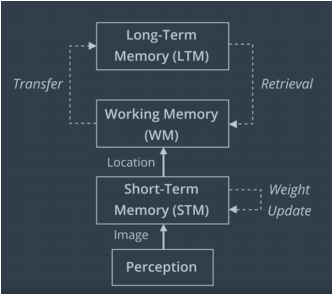
\includegraphics[width=\linewidth]{memory_management}
      \caption{ RTAB-MAP Memory Management}
      \label{fig:rtab_mem_mgmt}
\end{figure}


\section{SCENE AND MODEL CONFIGURATION}
\subsubsection{Robot Configuration}
The robot created is a race car. It was created by using the udacity bot and then by
adding front portion, a driver seat and a rear wing. The front wheels are simplified while
the back wheels are preserved. The laser sensor was placed on top of the driver seat, while
the camera is moved to the front of the car.
\begin{figure}[thpb]
      \centering
      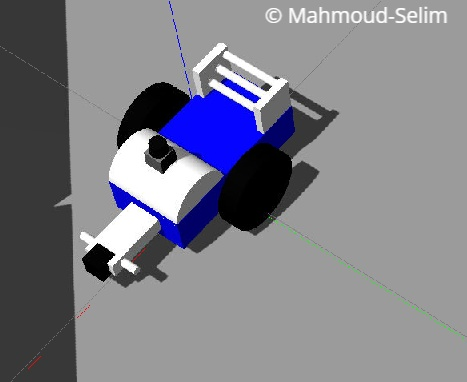
\includegraphics[width=\linewidth]{race car}
      \caption{race car.}
\end{figure}
\begin{figure}[thpb]
      \centering
      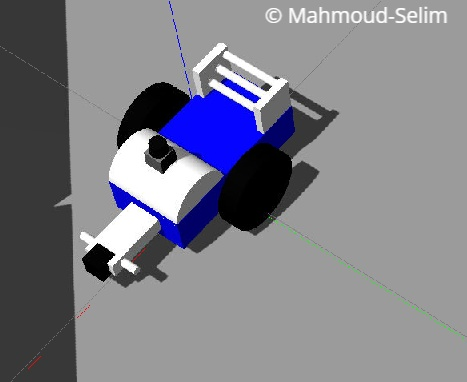
\includegraphics[width=\linewidth]{race car}
      \caption{race car tf frames.}
\end{figure}

\subsubsection{World Configuration}
\subsubsection {Kitchen Dining - Udacity World}
Mapping was done on two different worlds, first the
’kitchen and dining’ world provided by Udacity. There are
two small rooms, the kitchen with a table in the center and
a second smaller room.
\begin{figure}[thpb]
      \centering
      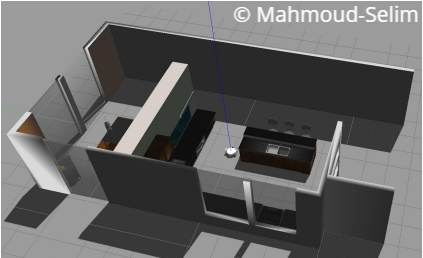
\includegraphics[width=\linewidth]{kitchen_dining}
      \caption{Kitchen Dining World}
\end{figure}

\subsubsection {Warehouse - My World}
The second world is a warehouse. It's like a large area square with many items and products in it. Mapping was done successfully and the 3D map did have the products in it successfully.
\begin{figure}[thpb]
      \centering
      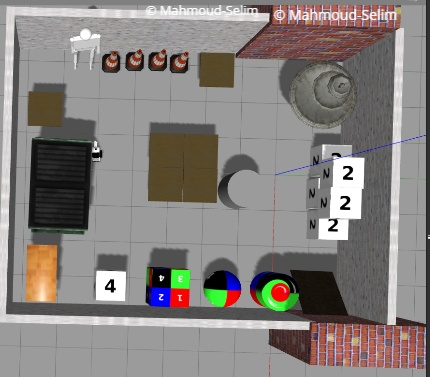
\includegraphics[width=\linewidth]{my_world}
      \caption{Kitchen Dining World}
\end{figure}

\section {Results}
\subsubsection {Mapping Kitchen and dining}
While mapping the kitchen and dining world, the robot
was able to map out the whole area with ease compared to
the second world, the smaller size of the environment and
its ample amount of features allowed RTABMap to detect
enough features after 2 cycles around the rooms to complete
the map. Bumping into walls or doing to many maneuvers
to unstuck the robot led to slight variations (objects not
appearing where they should be) in the map, but after a
few cycles the map corrected and realigned itself without
issues.
Global local closures were detected
during the mapping which was enough to fully map out
this environment.
\begin{figure}[thpb]
      \centering
      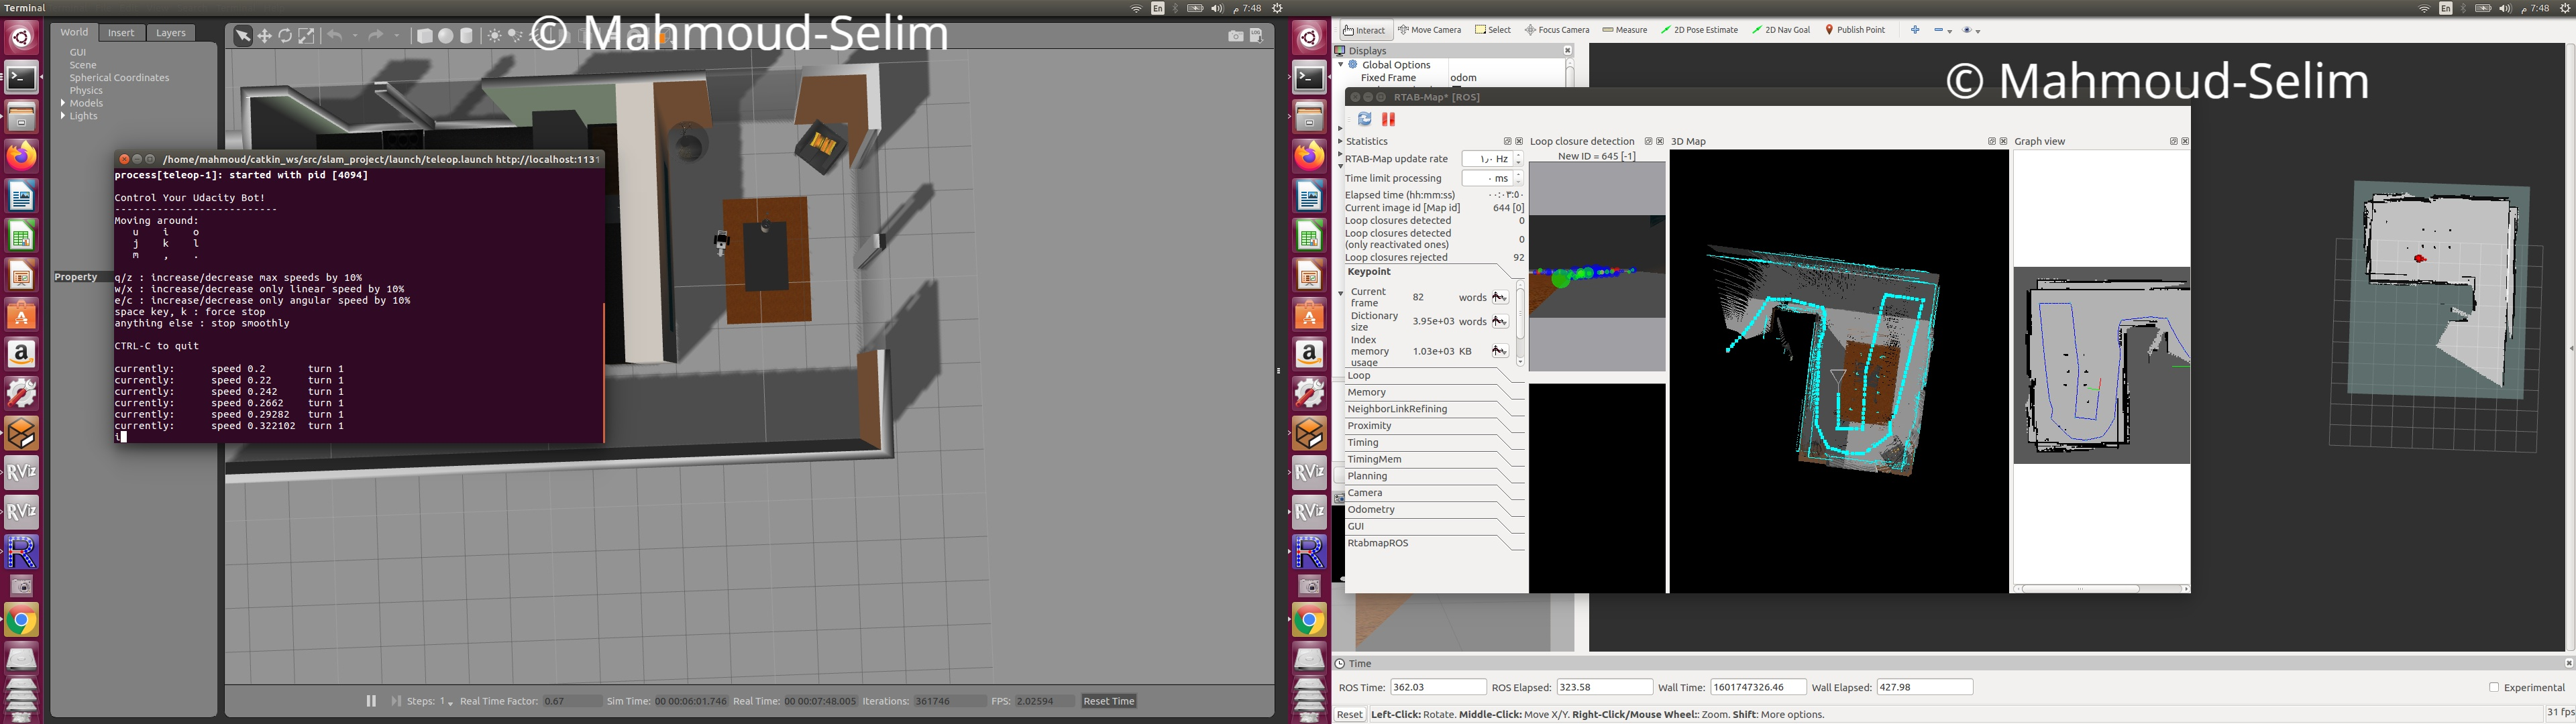
\includegraphics[width=\linewidth]{provided_world_partial_map}
      \caption{the map while mapping}
\end{figure}

\begin{figure}[thpb]
      \centering
      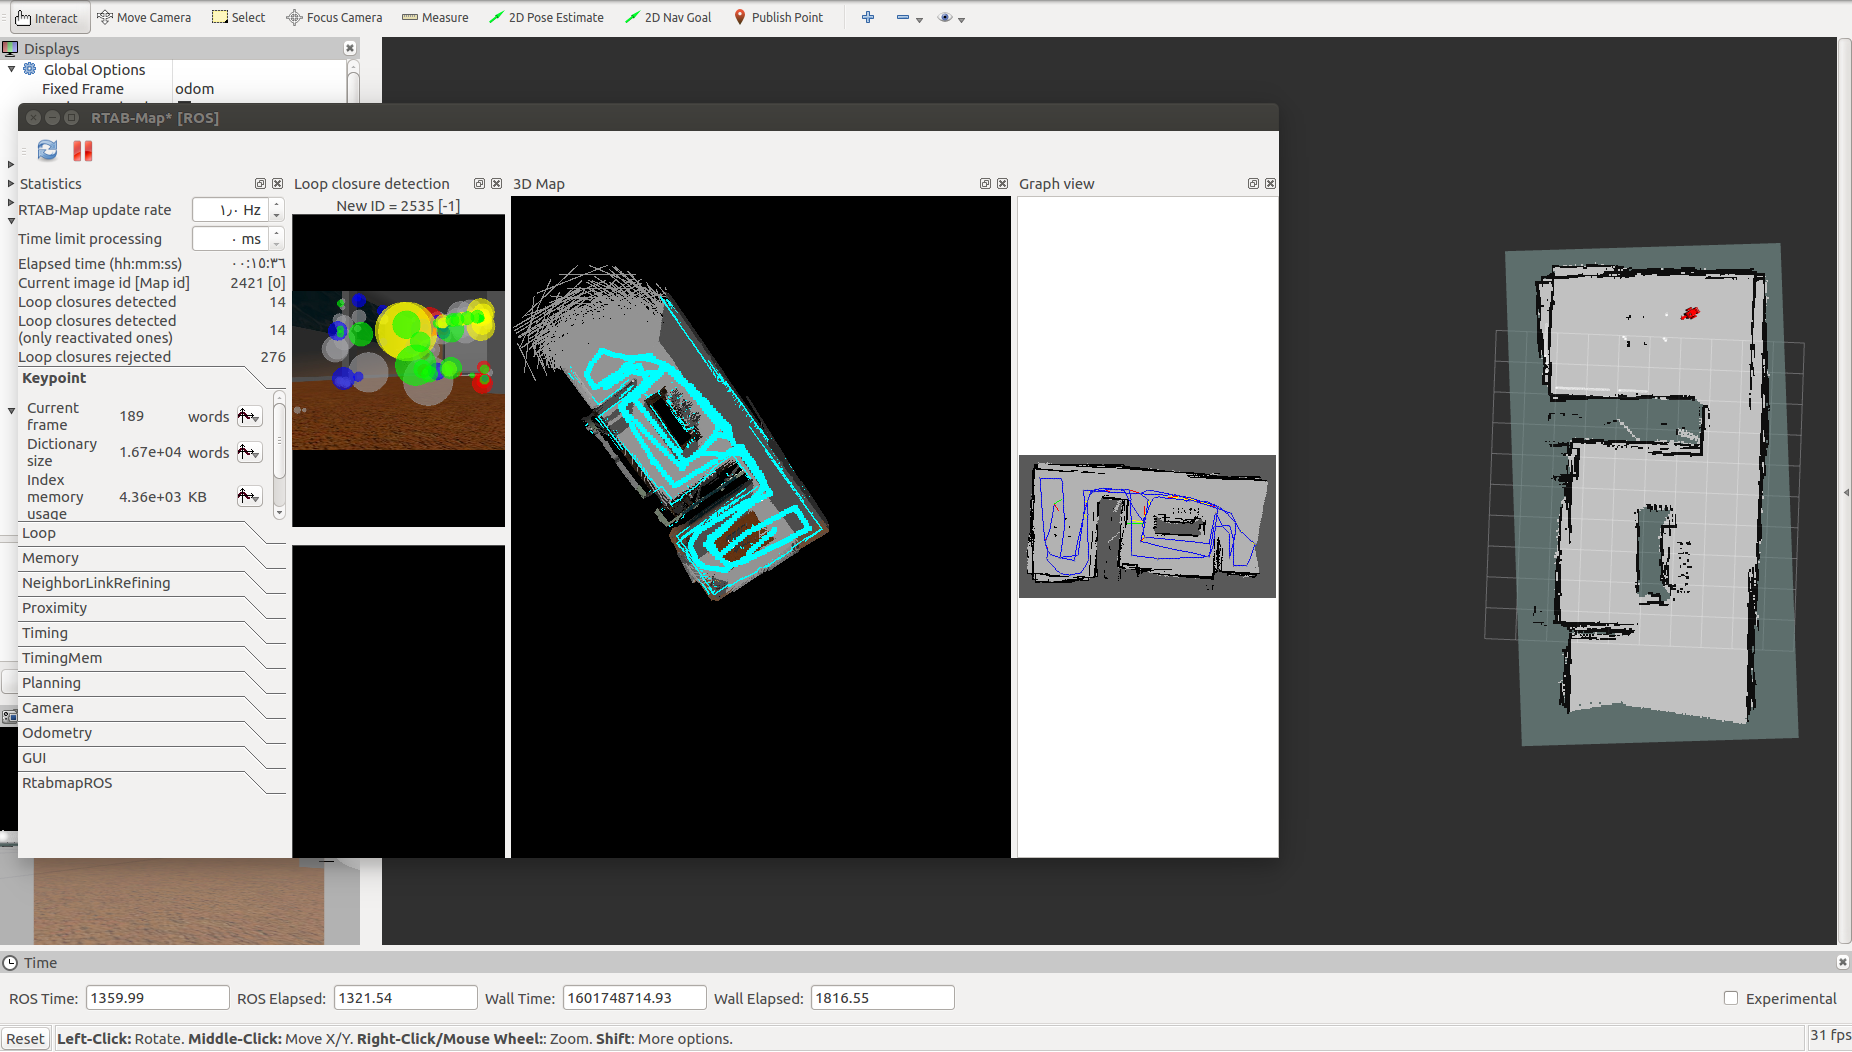
\includegraphics[width=\linewidth]{provided_world_full_map}
      \caption{the map after mapping.}
\end{figure}




\begin{figure}[thpb]
      \centering
      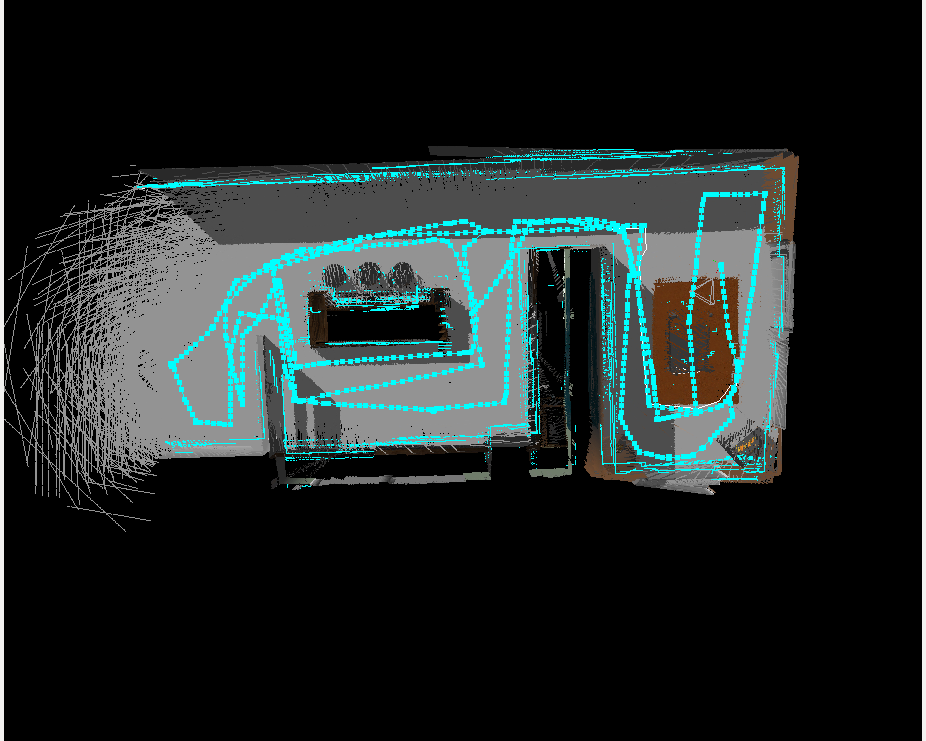
\includegraphics[width=\linewidth]{provided_world_3D_map}
      \caption{3D Map}
\end{figure}

\begin{figure}[thpb]
      \centering
      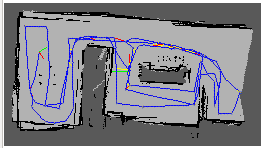
\includegraphics[width=\linewidth]{provided_world_2D_map}
      \caption{2D Map}
\end{figure}


\subsubsection {Mapping the warehouse (custom world)}
Same as before. the warehouse was mapped using the same algorithm with the same parameters. The robot did map the environment well. Figures of the mapped environment is shown below.
\begin{figure}[thpb]
      \centering
      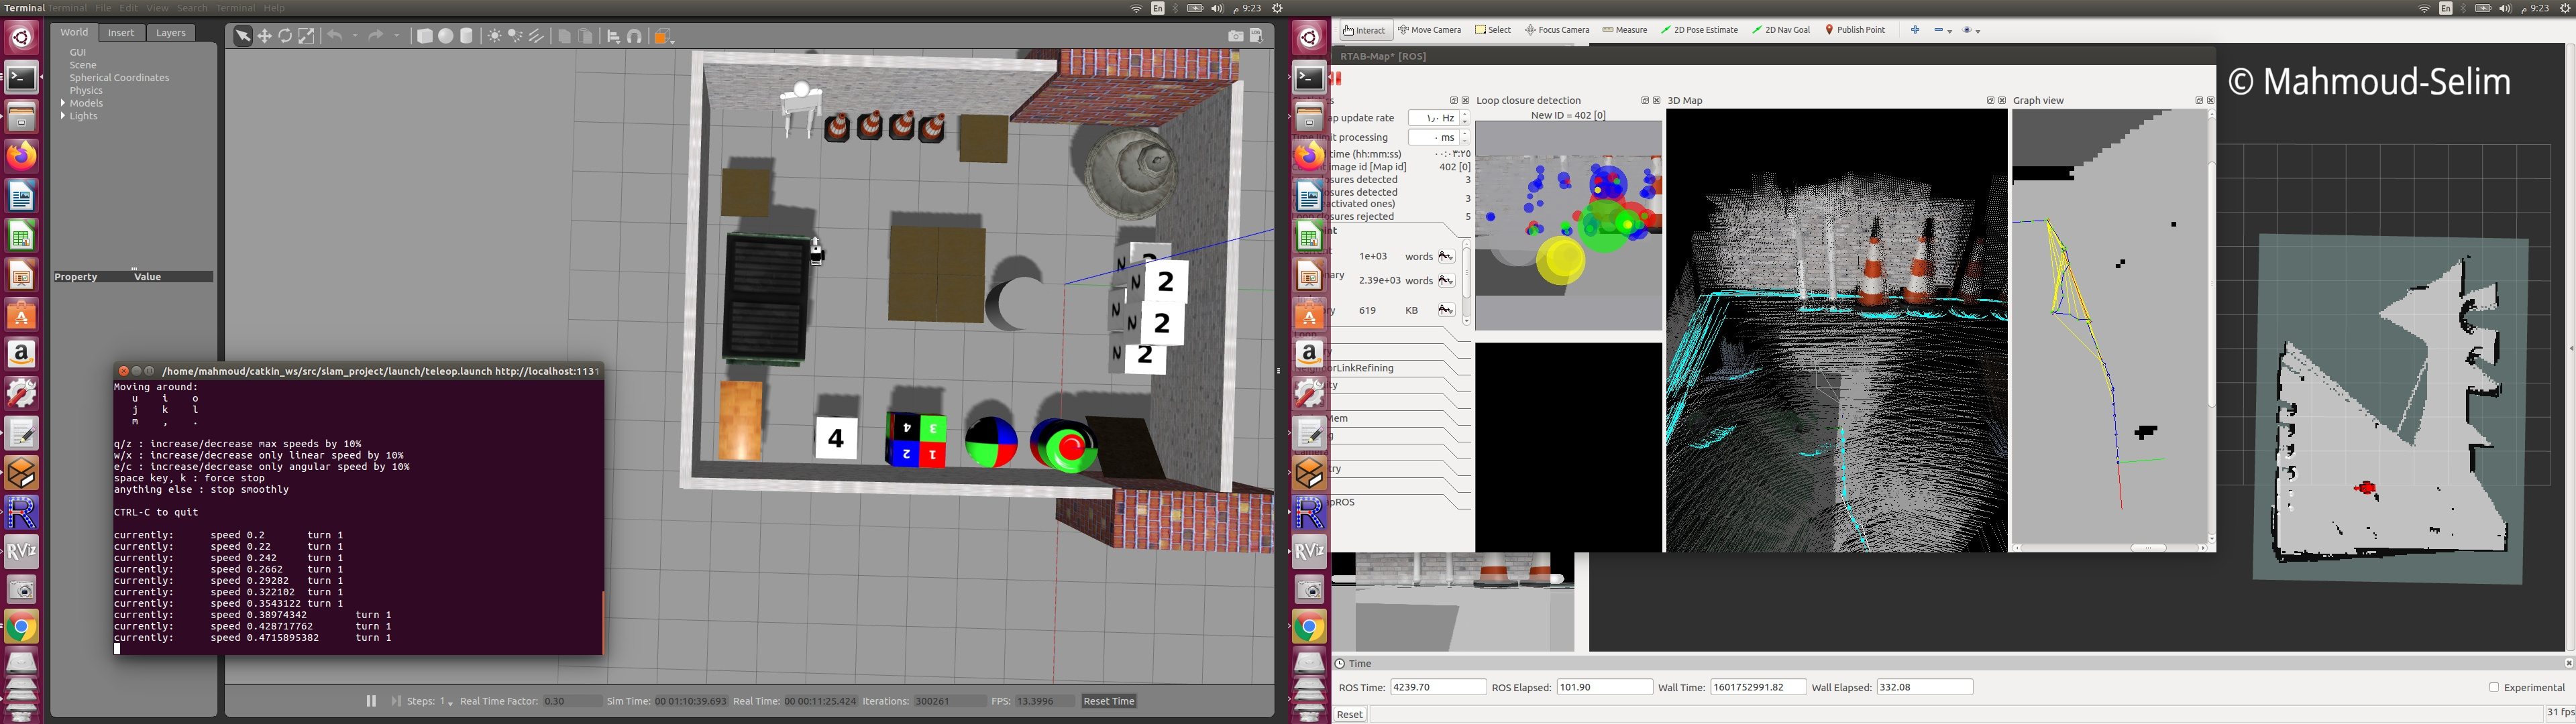
\includegraphics[width=\linewidth]{warehouse_world_partial_map}
      \caption{the map while mapping}
\end{figure}

\begin{figure}[thpb]
      \centering
      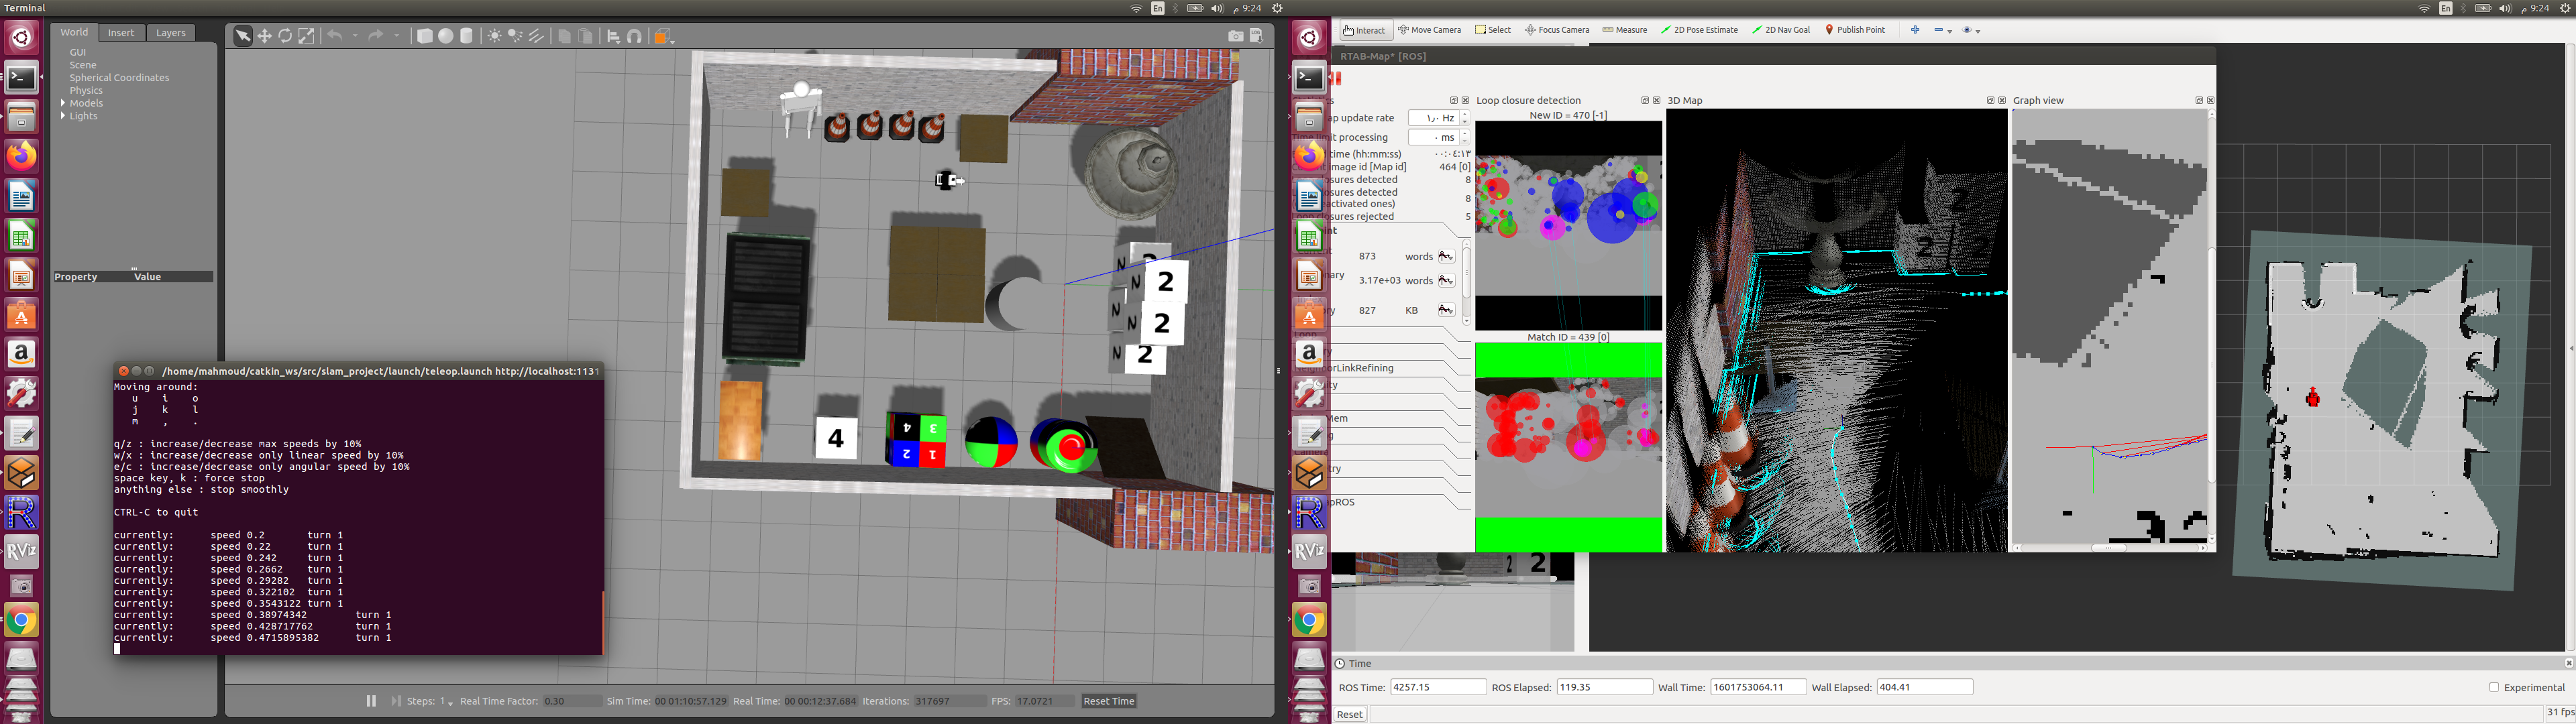
\includegraphics[width=\linewidth]{warehouse_world_2}
      \caption{the map while mapping.}
\end{figure}




\begin{figure}[thpb]
      \centering
      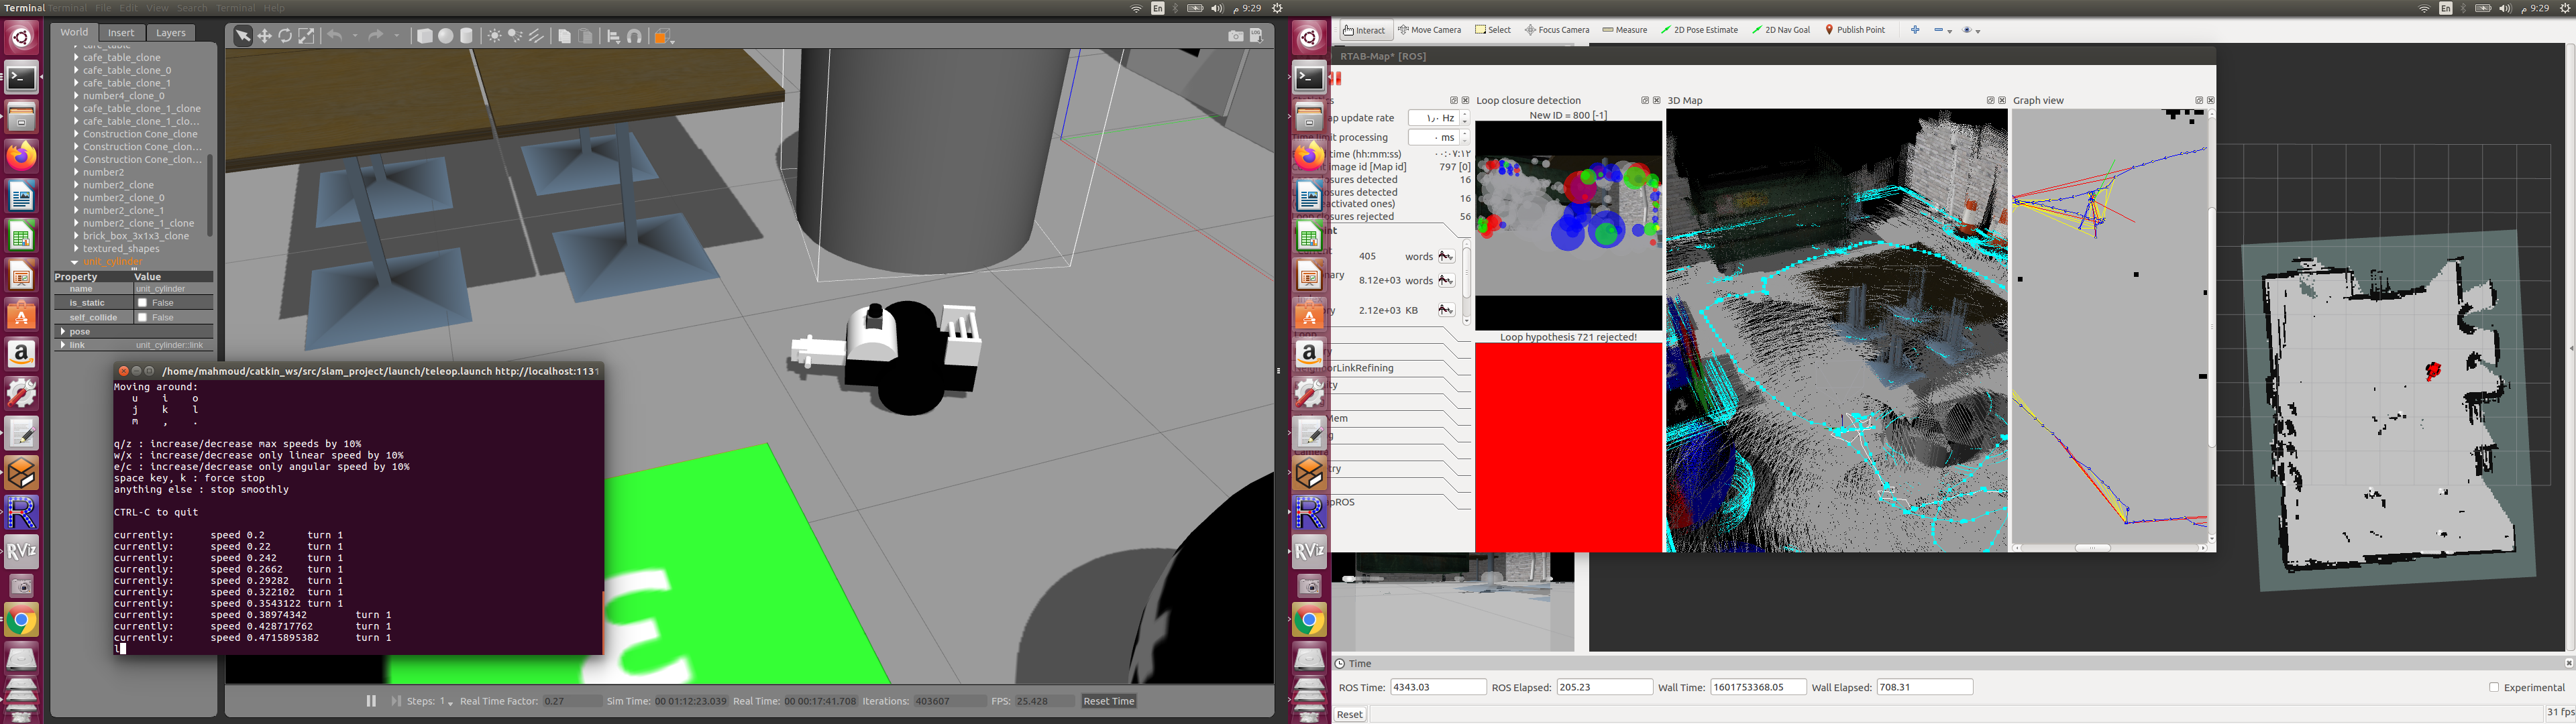
\includegraphics[width=\linewidth]{warehouse_world_full_map}
      \caption{the map after mapping.}
\end{figure}


\section{Discussion}
Mapping the two worlds raised a number of issues one
would have to consider when attempting to map environments. The first being that the robot used to do the
mapping needs to be tailored to the environment, from
its ability to navigate through the map, its speed and the
sensors used. Considering that both worlds were mapped
successfully, despite the issues with the robot, RTABMap
is able to recover, and can therefore be used in mapping
environments with less than ideal robots. However the
size (of the environment that is to be mapped compared
to the perceptual range of the robot), noise in perception and actuation, perceptual ambiguity (how similar different
places are, the more simlar different places can be, the higher
the perceptual ambiguity), and cycles can affect the robots
ability to map an environment without accumulating errors
past a certain threshold where the map would be unusable.
The size, could potentially be solved by either increasing
the number of robots or increasing the sensor’s range, or
both. For the noise in perception one could either improve the quality of the sensor or deepen the range of the
perceived by adding new types of sensors, for the noise
in actuation, then using rtabmap’s ability to get visual
odometry, which can be fused with the robot’s odometry
to improve the accuracy and therefore reduce the noise in
actuation. Perceptual ambiguity and cycles depend on the
map but their effects could be reduced by further tuning the
rtabmap’s parameters

\section{Conclusion / Future work}
Given the insightful results, RTABMap could be used on
robots to map any environments, and while more experimentations need to be done with regards to the way it
would interact with dynamic environments for instance, it
is safe to say that it is possible to use RTABMap to map real
environments using a laser scanner on a robot.
Future works would require upgrades on the robot,
switching to a 4-wheel based configuration will help with
the stability issues, and adding a pivot on the laser scanner
would reduce the number of maneuvers needed to fully
map out certain areas as stated previously. 

\bibliography{bib}
%\bibliographystyle{ieeetr}

\end{document}